\section{Pure Shift NMR}

In this section, a survey of some of the most prominent procedures for
producing pure shift spectra are presented.

\subsection{The \acl{2DJ} Experiment}
The \ac{2DJ} experiment\cite{Aue1976, Morris2009} provided the first means of
achieving pure shift spectra. It has a simple pulse sequence:
\[
    \ang{90} \xrightarrow{\nicefrac{\tone}{2}} \ang{180} \xrightarrow{\nicefrac{\tone}{2}} \ttwo.
\]
After excitation of magnetisation onto the transverse plane, the indirect
dimension evolution consists of a spin echo, with acquisition following
immediately afterwards. Fourier transformation in both dimensions leads to a
spectrum in which only scalar couplings contribute in $\Fone$, as the chemical
shifts are refocussed by the spin echo, while both scalar couplings and
chemical shifts contribute in $\Ftwo$.  \Iac{FID} generated by the \ac{2DJ}
experiment is hypercomplex, taking the form of \eqref{eq:general-fid} with
$D=2$ and $\zeta^{(1)} = \exp(\iu\cdot)$, i.e.
\begin{equation}%
    \begin{split}%
        y_{\none,\ntwo} =
        &\sum_{m=1}^{M} a_m \exp(\iu \phi_m)
            \exp\left(\left(2 \pi \iu \fonem - \etaonem\right) \none \Dtone\right) \times \\
        &\exp\left(\left(2 \pi \iu  \left(\ftwom - \foff\right)
            - \etatwom\right) \ntwo \Dttwo\right)
            + w_{\none,\ntwo}.
    \end{split}%
    \label{eq:jres-fid}
\end{equation}%
The transmitter offset term has been neglected in the indirect dimension, since
chemical shift evolution does not occur.
For each signal in the \ac{FID}, the indirect- and direct-dimension
frequencies are intimately linked. Consider a \ac{2DJ} dataset generated by a
spin system with $S$ distinct spins. The signals giving rise to a particular
spin $s \in \lbrace 1, \cdots, S \rbrace$ form a grouping $G_s
\subset \lbrace 1, \cdots, M \rbrace$. All of the signals in $G_s$
have (angular) frequencies given by
\begin{subequations}
    \begin{gather}
        2 \pi \fonem = \Updelta \omega_m,\\
        2 \pi \ftwom = \omega_{0,s} + \Updelta \omega_m,
    \end{gather}
    \label{eq:f1-f2-2dj}
\end{subequations}
$\forall m \in G_s$, where $\omega_{0,s}$ is the Larmor frequency of
the spin, and $\Updelta \omega_m$ is the displacement
of the signal from $\omega_{0,s}$, as a result of J-couplings\footnote{
    $\Updelta \omega_m$ will be a linear combination of all the scalar
    couplings associated with the spin giving rise to the signal, with all the
    coefficients being $\pm \nicefrac{1}{2}$.
}. Due to the relationship between the direct- and indirect-dimension
frequencies, all signals which are part of the same multiplet lie along
a line which bisects (i.e. makes a \ang{45} angle with) both the $\Fone$ and
$\Ftwo$ axes, as depicted in Figure \ref{fig:jres_spectrum}.a.
\begin{figure}%
    \centering%
    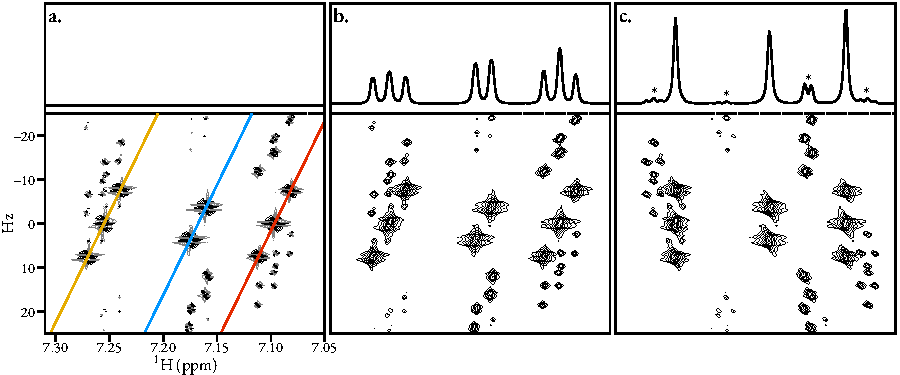
\includegraphics{jres_spectrum/jres_spectrum_new.pdf}%
    \caption[
        Region of a \acs{2DJ} spectrum of strychnine.
    ]
    {%
        Region of a simulated \acs{2DJ} spectrum of strychnine.
        Each panel depicts the spectrum following different processing
        procedures. Below: contour plots of the spectrum. Above: the
        summation of the spectrum along the indirect ($y$) axis.
        \textbf{a.} Spectrum produced by applying sine-bell apodisation
        followed by \ac{FT} in both dimensions.
        Coloured lines denote \ang{45} cross-sections along which the present
        multiplet structures lie.
        \textbf{b.} Magnitude-mode spectrum.
        \textbf{c.} Spectrum generated after application of a \ang{45} shear on
        the magnitude-mode spectrum. Peaks marked with asterisks panel c arise
        from the presence of strong coupling artefacts.
   }%
    \label{fig:jres_spectrum}%
\end{figure}%

One limitation of the \ac{2DJ} experiment is the fact that
spectra with pure absorption lineshapes cannot be produced. This is since, due
to the absence of a mixing period, it is not possible to produce a
complementary pair of phase- or amplitude-modulated \acp{FID}, which are
required to nullify dispersive contributions (see Section
\ref{subsec:mulitdim}).
The FT of a \ac{2DJ} \ac{FID} produces a spectrum with phase-twist
peaks (Figure \ref{fig:jres_spectrum}.a). As with other experiments which
produce hypercomplex signals, such as \ac{COSY}, the data is conventionally
displayed in ``magnitude-mode'' (Figure \ref{fig:jres_spectrum}.b) in which the
absolute value of each point in the spectrum is plotted.
A pure shift spectrum is generated from the \ac{2DJ} spectrum by performing a
\ang{45} shear\,---\,often referred to as a tilt\,---\,on the spectrum array,
leading to the separation of chemical shifts and scalar couplings onto
orthogonal axes (Figure \ref{fig:jres_spectrum}.c). Each slice through the
direct dimension of the \ac{2DJ} spectrum is subjected to a right circular
rotation such that
\begin{subequations}
    \begin{gather}
        s_{\none,\ntwo}^{\text{tilt}} =
            s_{\none,n^{(2)\prime}},\\
        n^{(2)\prime} = \left(\ntwo + \left\lfloor
                \frac
                    {\fswone \Ntwo\vpsub{\mathrm{sw}}}
                    {\fswtwo \None\vpsub{\mathrm{sw}}}
                \left(
                    \frac{\None\vpsub{\mathrm{sw}}}{2} - \none
                \right)
            \right\rceil
        \right) \bmod \Ntwo.
    \end{gather}
\end{subequations}
This achieves the mapping $s\left(\Fone,\Ftwo\right) \rightarrow s(\Fone, \Ftwo
- \Fone)$, which leads to a spectrum in which all peaks arising from a
given spin reside at the same direct-dimension frequency. The
effectiveness of the shear is maximised when both $\nicefrac{\fswtwo}{\fswone}$
and $\nicefrac{\Ntwo}{\None}$ are powers of 2\note{check this}. Summing the
sheared spectrum along $\Fone$ leads to the pure shift spectrum.
If the spectrum wasn't in magnitude-mode, shearing and summing would lead to
the absorptive and dispersive components of the spectrum cancelling each other
out, such that a vector of noise would be obtained.
With a magnitude-mode spectrum, the process leads to undesirable pure shift
spectra with broad ``wings'' on account of the presence of dispersive
character, and non-linearities. These effects can be suppressed by appropriate
processing to make the FID envelope symmetric in both dimensions, such as with
sine-bell apodisation or pseudo-echo reshaping\cite{Bax1981}, though this
results in a significant reduction in sensitivity being incurred.

Another feature which limits the effectiveness of the \ac{2DJ} experiment to
produce pure shift spectra are
\emph{strong coupling artefacts}\footnote{
    As stressed in \cite{Thrippleton2005}, these are not strictly artefacts,
    but rather genuine signals, which are expected to be present in the
    \ac{2DJ} dataset. Despite this, the term is widespread in the literature.
},
which arise due to mixing effects induced by the \ang{180} pulse in the
\ac{2DJ} sequence\cite{Wider1983,Thrippleton2005}. Examples of these are seen
in the spectra of Figure \ref{fig:jres_spectrum}, on account of the three spins
giving rise to the signals seen being strongly coupled. These artefacts always
have direct-dimension frequencies which match those of the conventional signals
in the spectrum\,---\,a feature which will be exploited in the \ac{CUPID}
procedure\,---\,however they do not lie along the same \ang{45} cross
sections. As a result, the final spectrum produced by shearing and summing will
feature extra low intensity signals that do not agree with the chemical shift
of a particular spin (see peaks marked with asterisks in Figure
\ref{fig:jres_spectrum}.c).

\subsection{The \acl{ZS} Method}
\label{subsec:ZS}
Zangger and Sterk introduced a pulse sequence element which achieves
\emph{slice-selective excitation}, by applying a low \ac{RF} power \ang{180}
pulse\footnote{Conventionally, a R-SNOB pulse is used\cite{Kupce1995}.} in the
presence of a \ac{PFG} along the $z$-axis\cite{Zangger1997}. Such an element
excites a
given spin only in a narrow range of heights in the sample, as the \ac{PFG}
induces a shift in resonance frequency according to $\Updelta \omega(z) = \gamma
gz$, where $g$ is the magnitude of the \ac{PFG}. By placing a hard
\ang{180} pulse adjacent to the selective pulse, the
``active'' spin in a given slice is rotated by \ang{360} (i.e. no net
rotation), while all other (``passive'') spins are only rotated by \ang{180}.
Placing such a element in the middle of the $\tone$ evolution therefore
achieves refocussing of the J-couplings associated with the active
spin\cite{Aguilar2010}. In order to achieve effective decoupling of any given
pair of spins, it is necessary that the bandwidth of the selective π-pulse is
smaller than the difference in their Larmor frequencies. However, with more
selective pulses, a smaller proportion of the available spin magnetisation will
contribute to the final FID, and hence sensitivity will be diminished
\footnote{
    The reduction in sensitivity is $\propto \nicefrac{\Updelta F}{\gamma g l_z}$,
    where $\Updelta F$ is the selective pulse bandwidth, and $l_z$ is the length of
    the sample lying within the receiver coil ($\approx
    \qty{1.5}{\centi\meter}$).
}.
Therefore a trade-off exists between effective decoupling of all spins, and
achieving the greatest sensitivity possible. In the case of strong coupling,
the \ac{ZS} method tends to perform poorly relative to other options for this
reason. The \ac{ZS} element has been utilised in order to generate \ac{2DJ}
datasets comprising phase-modulated pairs, enabling the generation of pure
absorption-mode spectra\cite{Pell2007}. Pure shift spectra with far more
desirable lineshapes can be achieved relative to using a typical magnitude-mode
spectrum \ac{2DJ}, though with a significant loss of sensitivity.

\subsection{The \acs{BIRD} Method}
The \ac{BIRD} pulse sequence element\cite{Garbow1982,Bax1983} also takes
advantage of the idea of selectively inverting passive spins, while leaving
active spins unaffected.
However the active spins are those which are directly bound to a low natural
abundance
heteronucleus, with the two most common heteronuclei used being
\textsuperscript{13}C (1.1\% abundance) and \textsuperscript{15}N (0.37\%
abundance).
The passive spins are those bound to far more abundant nucleus (i.e.
\textsuperscript{12}C or \textsuperscript{14}N). The reduction in sensitivity
of the experiment relative to a full-sensitivity experiment is therefore known
and constant across samples. In scenarios where strong coupling exists, \ac{BIRD} can
achieve improved sensitivity over \ac{ZS}, since with the latter a very weak
selective pulse would be required to ensure it is of a sufficiently small
bandwidth. The \ac{BIRD} method is particularly attractive in scenarios where
the sensitivity penalty due to the involvement of a low-abundance nucleus has
already been paid, for example in sequences where an \ac{INEPT} element is
present\cite{Paudel2013}.

\subsection{\acs{PSYCHE}}
\label{subsec:psyche}
The most recent major development in pure shift spectroscopy is the \ac{PSYCHE}
experiment\cite{Foroozandeh2014,Foroozandeh2018}.
\note{Description... Element, How it works (very simple), Effectiveness}

The \ac{PSYCHE} element has also been employed in conjunction with the \ac{2DJ}
experiment in order to produce spectra which already feature orthogonal
separation of the chemical shifts and couplings along the two frequency
axes\cite{Foroozandeh2015,Kiraly2017}. Being a 3D experiment, the
\ac{PSYCHE}-\ac{2DJ} requires long experiment times (typically tens of hours)
in order to produce a spectrum with well-resolved multiplet structures in the
indirect dimension.

\subsection{Pure shift spectra from 2DJ estimation}
\note{Mandelstahm?}

Beyond specialised pulse sequences, procedures based on the estimation of
\ac{2DJ} datasets have also been developed to achieve broadband homodecoupling.
Nuzillard introduced \ac{ALPESTRE}\cite{Nuzillard1996,Martinez2012}, in which
the parameters of each indirect-dimension FID are estimated using \ac{LPSVD},
such that a set of parameters $\symbf{\Theta} \in \mathbb{R}^{\Ntwo
\times 4M}$ is generated.
\begin{equation}
    \symbf{\theta}_{\ntwo} =
    \begin{bmatrix}
        \bda_{\ntwo}\T &
        \bdphi_{\ntwo}\T &
        \bdf_{\ntwo}\T &
        \bdeta_{\ntwo}\T
    \end{bmatrix}\T.
\end{equation}
The parameters generated are used to propagate each FID backward into
$-\tone$, producing a ``full-echo'':
\begin{equation}
    \begin{split}
        y^{\text{full}}_{\none,\ntwo} = \sum_{m=1}^{M}
            a_{\ntwo,m}
            \exp(\iu \phi_{\ntwo,m})
            \exp\left(\left(2 \pi \iu f_{\ntwo,m} \none
            -\eta_{\ntwo,m}  \left\lvert \none \right\rvert \right)\Dtone\right), \\
        \forall \none \in \lbrace -\None + 1, \cdots, 0, \cdots, \None - 1 \rbrace,\ \forall \ntwo \lbrace 0, \cdots, \Ntwo - 1 \rbrace.
    \end{split}
    \label{eq:full-echo}
\end{equation}
\ac{FT} of \eqref{eq:full-echo} generates a spectrum whose real component comprises absorption-mode
Lorentzian character in both dimensions. This opens up the means of producing
pure-shift spectra from the \ac{2DJ} experiment with sharp lineshapes and
without signal loss. A similar approach proposed by Mutzenhardt et al.
instead constructs full echoes via \ac{LP} of each direct-dimension
\ac{FID}, and generates a full echo by propagating into
$-\ttwo$\cite{Mutzenhardt1999}.


